% ---------------------------------------------------------------
% TEMPLATE TCC1 - SENAC SANTO AMARO
% ---------------------------------------------------------------
% Trabalho de Conclusão de Curso 1
% Elaborado para apresentação da proposta inicial do TCC
% Estrutura: 4 capítulos (Introdução, Revisão Bibliográfica,
%            Desenvolvimento, Referências Bibliográficas)
% ---------------------------------------------------------------

\documentclass[
    12pt,                % tamanho da fonte
    openright,           % capítulos começam em página ímpar
    oneside,             % para impressão em apenas um lado do papel
    a4paper,             % tamanho do papel
    english,             % idioma adicional
    brazil               % idioma principal
]{abntex2}

% ---------------------------------------------------------------
% PACOTES
% ---------------------------------------------------------------
\usepackage{lmodern}                % Fonte Latin Modern
\usepackage[T1]{fontenc}            % Seleção de códigos de fonte
\usepackage[utf8]{inputenc}         % Codificação do documento
\usepackage{lastpage}               % Usado pela Ficha catalográfica
\usepackage{indentfirst}            % Indenta o primeiro parágrafo
\usepackage{color}                  % Controle de cores
\usepackage{graphicx}               % Inclusão de gráficos
\usepackage{microtype}              % Melhorias de justificação
\usepackage{float}                  % Para posicionamento de figuras
\usepackage{booktabs}               % Tabelas profissionais
\usepackage{multirow}               % Células mescladas em tabelas
\usepackage{longtable}              % Tabelas longas
\usepackage{amsmath,amssymb}        % Símbolos matemáticos
\usepackage{pgfgantt}               % Diagramas de Gantt
\usepackage[brazilian,hyperpageref]{backref}  % Páginas com citações
\usepackage[alf]{abntex2cite}       % Citações ABNT
\usepackage{tikz}
\usepackage{tabularx}
\usetikzlibrary{shapes.geometric, arrows, positioning, calc}
\usepackage{tikz}
\usetikzlibrary{shapes.geometric, arrows.meta, positioning}

% ---------------------------------------------------------------
% CONFIGURAÇÕES DO PDF
% ---------------------------------------------------------------
\makeatletter
\hypersetup{
    pdftitle={\@title},
    pdfauthor={\@author},
    pdfsubject={TCC1 - SENAC Santo Amaro},
    pdfcreator={LaTeX with abnTeX2},
    pdfkeywords={tcc}{senac}{santo amaro}{trabalho de conclusão},
    colorlinks=true,        % false: links em caixas; true: links coloridos
    linkcolor=senacblue,    % cor dos links internos
    citecolor=senacblue,    % cor dos links para bibliografia
    filecolor=magenta,      % cor dos links para arquivos
    urlcolor=senacblue,
    bookmarksdepth=4
}
\makeatother

% ---------------------------------------------------------------
% CONFIGURAÇÕES DE APARÊNCIA DO PDF FINAL
% ---------------------------------------------------------------
\definecolor{senacblue}{RGB}{41,5,195}

% ---------------------------------------------------------------
% INFORMAÇÕES DO DOCUMENTO
% ---------------------------------------------------------------
\titulo{Análise Experimental da Inferência SepConv em C++ com Ênfase em Eficiência Computacional e Uso de VRAM}
\autor{Pedro Henrique Gomes}
\local{São Paulo}
\data{2026}
\orientador{Prof. Afonso Brandão}

\instituicao{%
  SENAC -- Serviço Nacional de Aprendizagem Comercial
  \par
  Unidade Santo Amaro
  \par
  Curso de Bacharelado em Ciência da Computação
}

\tipotrabalho{Trabalho de Conclusão de Curso I}

\preambulo{Proposta de Trabalho de Conclusão de Curso apresentado ao SENAC Santo Amaro como requisito parcial para aprovação na disciplina de TCC1 do curso de Bacharelado em Ciência da Computação.}

% ---------------------------------------------------------------
% COMPILA O ÍNDICE
% ---------------------------------------------------------------
\makeindex

% ---------------------------------------------------------------
% INÍCIO DO DOCUMENTO
% ---------------------------------------------------------------
\begin{document}

% Seleciona o idioma do documento
\selectlanguage{brazil}

% Retira espaço extra obsoleto entre as frases
\frenchspacing

% ---------------------------------------------------------------
% ELEMENTOS PRÉ-TEXTUAIS
% ---------------------------------------------------------------
\pretextual

% ---------------------------------------------------------------
% CAPA
% ---------------------------------------------------------------
\imprimircapa

% ---------------------------------------------------------------
% FOLHA DE ROSTO
% ---------------------------------------------------------------
\imprimirfolhaderosto

% ---------------------------------------------------------------
% RESUMO
% ---------------------------------------------------------------
\begin{resumo}
A crescente disseminação de dispositivos de exibição com elevadas taxas de atualização (60 Hz a 144 Hz) evidenciou a limitação temporal de conteúdos audiovisuais capturados nas frequências tradicionais de 24 FPS a 30 FPS. Para mitigar artefatos visuais e aumentar a fluidez contínua, a Interpolação de Quadros de Vídeo (VFI -- \textit{Video Frame Interpolation}) busca sintetizar quadros intermediários. Embora abordagens baseadas em fluxo óptico denso, como o modelo RAFT, alcancem elevada precisão, a alta complexidade computacional e a dependência de \textit{frameworks} de alto nível (PyTorch) limitam sua aplicação sob restrições severas de hardware. Como alternativa eficiente, as Convoluções Adaptativas Separáveis tratam a síntese como uma filtragem local adaptativa, decompondo \textit{kernels} bidimensionais $N \times N$ em dois filtros unidimensionais $1D$, reduzindo a complexidade aritmética de $O(N^2)$ para $O(2N)$ por pixel. Este trabalho apresenta uma análise experimental do modelo SepConv através da implementação de um motor de inferência nativo em C++ e CUDA, desacoplado de ecossistemas de treinamento. O \textit{pipeline} proposto integra a biblioteca OpenCV para entrada e saída de dados, a API C++ do ONNX Runtime para a extração dos vetores de movimento e \textit{kernels} customizados em CUDA para a execução paralela das convoluções mantidas diretamente na memória de vídeo (VRAM). A validação experimental prevê a avaliação do compromisso entre o consumo de memória VRAM (aferido via NVML e focado em GPUs de consumo de 8 GB), a latência de execução em milissegundos e a fidelidade visual (mensurada por PSNR e SSIM sobre o \textit{dataset} Vimeo-90K). Os resultados buscam comprovar a viabilidade técnica do controle granular de memória para viabilizar a interpolação de vídeos em alta definição em hardwares comerciais restritos.

\vspace{\onelineskip}

\noindent
\textbf{Palavras-chave}: Interpolação de Quadros de Vídeo. Convoluções Adaptativas Separáveis. C++. CUDA. Otimização de VRAM. SepConv.
\end{resumo}

% ---------------------------------------------------------------
% SUMÁRIO
% ---------------------------------------------------------------
\pdfbookmark[0]{\contentsname}{toc}
\tableofcontents
\cleardoublepage

% ---------------------------------------------------------------
% ELEMENTOS TEXTUAIS
% ---------------------------------------------------------------
\textual

% ===============================================================
% CAPÍTULO 1 - INTRODUÇÃO
% ===============================================================

\chapter{Introdução}
\label{cap:introducao}

Historicamente, os sistemas de captura e exibição de imagens em movimento foram limitados pela capacidade mecânica e elétrica dos dispositivos da época. Durante a consolidação do cinema sonoro no início do século XX, a taxa de aproximadamente 24 quadros por segundo (FPS) tornou-se um padrão industrial por representar um equilíbrio entre fluidez perceptiva e custo de armazenamento e reprodução do filme físico \cite{Bordwell2016}. Taxas nessa faixa passaram a ser suficientes para produzir a percepção de movimento contínuo ao sistema visual humano, reduzindo a percepção de descontinuidade temporal durante a projeção \cite{Watkinson2009}.

Com a evolução tecnológica dos dispositivos de exibição, monitores e televisores modernos passaram a operar em frequências significativamente superiores, variando entre 60 Hz e 144 Hz. Entretanto, grande parte do conteúdo audiovisual disponível ainda permanece limitada às taxas tradicionais de captura, como 24 FPS ou 30 FPS, criando uma discrepância entre a capacidade de atualização do hardware atual e a quantidade de informação temporal presente no vídeo original. Essa diferença entre a taxa de amostragem temporal do conteúdo original e a frequência de atualização do dispositivo de exibição resulta no fenômeno conhecido como subamostragem temporal. De acordo com Watkinson (2009) e Szeliski (2022), a incapacidade de fornecer amostras intermediárias suficientes durante movimentos rápidos reduz a percepção de continuidade temporal pelo sistema visual humano, induzindo a artefatos perceptuais como tremulação de movimento (\textit{motion judder}), borramento dinâmico e quebra na percepção de fluidez contínua.

Nesse contexto, a Interpolação de Quadros de Vídeo (VFI -- Video Frame Interpolation) surge como uma técnica essencial para sintetizar quadros intermediários artificialmente, aumentando a fluidez temporal do conteúdo exibido. Tradicionalmente, a literatura divide as abordagens de VFI em métodos baseados em fluxo óptico, como o modelo RAFT \cite{Teed2020}, e métodos baseados em kernels. Embora modelos de aprendizado profundo tenham atingido patamares elevados de precisão, eles frequentemente demandam recursos computacionais extensivos e dependem de frameworks pesados, o que limita sua aplicação em cenários de hardware restrito ou escassez de memória RAM e VRAM.
Para mitigar a alta demanda de recursos computacionais, representada pelo elevado volume de operações de ponto flutuante (FLOPs), pelo esgotamento do armazenamento de tensores na memória de vídeo (VRAM) e pela alta latência de execução ---, a literatura recente busca alternativas mais eficientes aos modelos tradicionais de fluxo óptico. Em cenários de hardware restrito, típicos de computadores pessoais e dispositivos de consumo doméstico dotados de GPUs comerciais limitadas a 8 GB de VRAM, a execução de ecossistemas densos baseados em \textit{frameworks} de alto nível (como PyTorch) torna-se inviável em altas resoluções. Nesse contexto, Niklaus et al. (2017) propuseram a utilização de Convoluções Adaptativas Separáveis, técnica que decompoe \textit{kernels} bidimensionais $N \times N$ em pares de filtros unidimensionais $1D$, reduzindo a complexidade computacional de $O(N^2)$ para $O(2N)$. A implementação dessa etapa de inferência em linguagem de baixo nível (C++/CUDA) possibilita um controle granular sobre o gerenciamento de memória gráfica, permitindo isolar a eficiência do algoritmo e testar sua viabilidade em computadores comuns.
Diante desse gargalo tecnológico entre a necessidade de fluidez em computadores pessoais e as limitações físicas de memória do hardware de consumo, formaliza-se a seguinte \textbf{hipótese científica}: postula-se que a separabilidade matemática dos \textit{kernels}, quando associada a um \textit{pipeline} de inferência nativo em C++ e CUDA (desacoplado de \textit{frameworks} de treinamento), reduz o pico de consumo de VRAM e a latência de execução em comparação às implementações de alto nível em Python/PyTorch. A partir dessa premissa, o presente trabalho tem como objetivo avaliar a viabilidade técnica do processamento de vídeos em alta definição sob o limite de 8 GB de VRAM, investigando o equilíbrio entre a eficiência computacional no hardware do usuário final e a fidelidade visual dos quadros sintetizados.

% ---------------------------------------------------------------
\section{Contexto}
\label{sec:contexto}

Historicamente, os padrões de captura e transmissão de vídeo foram consolidados sob limitações técnicas de largura de banda e processamento da época, estabelecendo taxas como 24 ou 30 quadros por segundo (FPS) como normas globais \cite{Gonzalez2009}. Contudo, a evolução recente dos dispositivos de exibição permitiu o surgimento de telas com altas taxas de atualização (60Hz a 144Hz), criando uma disparidade entre o conteúdo disponível e a capacidade do hardware. Essa lacuna resulta em uma percepção de movimento descontínua, pois a amostragem temporal reduzida do conteúdo original não preenche os intervalos de atualização das telas modernas, comprometendo a fluidez visual esperada pelo usuário.

Diferente de métodos simplificados de amostragem de quadros, a VFI busca sintetizar um novo quadro no instante $t+0.5$ por meio de uma combinação ponderada de informações espaciais e temporais das imagens adjacentes. Esse processo considera o contexto do movimento e a correlação entre pixels \cite{Niklaus2017}. Ao elevar a taxa de quadros por segundo, a técnica objetiva atenuar artefatos de movimento na percepção humana.

Entretanto, a implantação prática desses algoritmos enfrenta barreiras atreladas ao custo computacional espacial e aritmético. Modelos de estado da arte demandam alto armazenamento de tensores intermediários na memória de vídeo (VRAM), limitando frequentemente sua execução a hardwares de alto desempenho \cite{Bao2019}. A transposição de modelos matemáticos para pipelines de inferência otimizados surge como um caminho científico relevante para avaliar os reais gargalos de desempenho em sistemas com memória de consumo limitada.

% ---------------------------------------------------------------

\section{Justificativa}
\label{sec:justificativa}

A escolha pela implementação de algoritmos de interpolação baseados em Convoluções Adaptativas Separáveis justifica-se, primordialmente, pela necessidade de viabilizar a fluidez visual em sistemas de computação pessoal com recursos de memória limitados. Enquanto as abordagens de convolução espacial completa exigem uma complexidade quadrática de $N^2$ operações por pixel para a síntese de quadros, a técnica de decomposição em \textit{kernels} unidimensionais reduz esse custo para uma ordem linear de $2N$ \cite{Niklaus2017}. Essa eficiência matemática busca diminuir o tempo de execução e, essencialmente, o \textit{footprint} (consumo espacial) na memória de vídeo (VRAM), viabilizando que hardwares de consumo processem sequências de vídeo em alta definição sem estourar os limites da placa gráfica.

A delimitação experimental em GPUs de consumo dotadas de 8 GB de memória VRAM fundamenta-se na ampla representatividade desse perfil de hardware no mercado do usuário final. Segundo os levantamentos da \textit{Steam Hardware \& Software Survey} \cite{SteamSurvey2026}, placas de vídeo com 8 GB de VRAM representam aproximadamente 26\% das configurações ativas na plataforma, constituindo a capacidade individual mais expressiva entre os usuários domésticos. Embora modelos de alto desempenho com 16 GB ou mais tenham registrado crescimento recente, a faixa de 8 GB permanece como a principal barreira física para a execução de modelos densos de inteligência artificial em ambientes não corporativos.

Sob a perspectiva da Ciência da Computação e da Engenharia de Software, a pesquisa justifica-se pela investigação do gargalo de abstração imposto por \textit{frameworks} de alto nível (como Python/PyTorch). Embora adequados para prototipagem e treinamento, esses ecossistemas introduzem \textit{overheads} significativos decorrentes do gerenciamento dinâmico de memória, da alocação redundante de tensores temporários e da camada de interpretação do runtime. Ao transpor a etapa de inferência do modelo SepConv diretamente para a linguagem C++, integrada ao ecossistema nativo ONNX Runtime e a \textit{kernels} customizados em CUDA, é possível exercer um controle determinístico sobre a alocação e transferência de ponteiros na VRAM. 

Dessa forma, o trabalho busca demonstrar como o gerenciamento granular de hardware e a otimização algorítmica de baixo nível conseguem mitigar limitações físicas de memória gráfica, oferecendo um ponto de equilíbrio viável entre a qualidade perceptual da imagem e o desempenho computacional em sistemas comerciais.

% ---------------------------------------------------------------
\section{Objetivo}
\label{sec:objetivo}

Esta seção delimita o escopo técnico da pesquisa, focando na avaliação de desempenho sob restrições físicas de VRAM em hardware de consumo.

\subsection{Objetivo principal}

Avaliar experimentalmente os efeitos da convolução separável no desempenho computacional da inferência do modelo SepConv em GPU, utilizando uma implementação nativa em C++, com ênfase na latência e no consumo de memória VRAM em hardware de consumo.

\subsection{Objetivos secundários}

\begin{enumerate}
    \item Desenvolver um fluxo de processamento em C++ e OpenCV para a extração de quadros e transferência eficiente para a memória da placa de vídeo;
    \item Integrar a biblioteca \textit{ONNX Runtime} em C++ para carregar os pesos pré-treinados do modelo SepConv e inferir os vetores separáveis (1D) correspondentes ao movimento;
    \item Codificar e otimizar \textit{kernels} customizados em arquitetura CUDA para aplicar a operação de convolução separável diretamente na VRAM;
    \item Comparar o desempenho da implementação proposta (C++) exclusivamente com a \textit{baseline} da implementação original do SepConv (Python/PyTorch), com ênfase na aferição da redução do pico de consumo de memória VRAM e na latência de execução;
    \item Mensurar o custo computacional e a viabilidade de execução com baixa latência, analisando o tempo de execução, a taxa de quadros por segundo (FPS) e o pico de uso de memória VRAM em hardware de consumo para diferentes resoluções de vídeo.
\end{enumerate}

% ===============================================================
% CAPÍTULO 2 - REVISÃO BIBLIOGRÁFICA
% ===============================================================
\chapter{Revisão Bibliográfica}
\label{cap:revisao}

A revisão bibliográfica tem como finalidade apresentar o embasamento teórico do trabalho, demonstrando o conhecimento do autor sobre o tema e identificando o estado da arte. Este capítulo deve ser organizado por conceitos e temas, construindo uma linha de argumentação que sustente a proposta do trabalho.

% ---------------------------------------------------------------
\section{Metodologia da pesquisa bibliográfica}
\label{sec:metodologia_pesquisa}

A pesquisa bibliográfica foi conduzida por meio de buscas nas bases Google Scholar e IEEE Xplore, utilizando combinações de palavras-chave relacionadas ao tema da pesquisa. As consultas empregaram operadores lógicos para refinar os resultados, buscando trabalhos relacionados à interpolação de quadros de vídeo, convoluções separáveis, fluxo óptico e otimização de inferência em GPU.

\begin{itemize}
    \item \textbf{Bases de dados consultadas}: Google Scholar e IEEE Xplore;

    \item \textbf{Palavras-chave utilizadas}: 
    \begin{itemize}
        \item ("video frame interpolation" OR "frame interpolation") AND ("convolutional neural network" OR CNN OR convolution) AND (video OR image sequence);
        \item ("video frame interpolation") AND (convolution OR "adaptive convolution" OR "separable convolution");
        \item ("video frame interpolation") AND ("optical flow" OR convolution OR transformer OR "deep learning");
    \end{itemize}
\end{itemize}

\subsection{Período de abrangência}

Embora as buscas tenham retornado publicações de diferentes períodos, foi adotado como critério principal a seleção de trabalhos publicados a partir de 2015. Esse recorte temporal foi definido por contemplar o surgimento e a consolidação das principais técnicas modernas de aprendizado profundo aplicadas à interpolação de quadros de vídeo. Trabalhos anteriores foram mantidos apenas quando considerados referências clássicas ou fundamentais para a compreensão dos conceitos teóricos utilizados nesta pesquisa.

O processo de busca inicial retornou aproximadamente 5.000 resultados. Em uma primeira etapa de triagem (\textit{screening}), foi realizada a leitura dos títulos dos trabalhos encontrados, resultando na seleção de aproximadamente 60 publicações potencialmente relevantes ao tema investigado. Após a aplicação do filtro temporal, cerca de 20 artigos permaneceram para análise.

Na etapa seguinte, foi realizada a leitura dos resumos dos trabalhos selecionados, reduzindo o conjunto para aproximadamente 12 publicações. Por fim, foi conduzida uma leitura mais aprofundada dos artigos com maior aderência ao escopo da pesquisa, dos quais cerca de cinco foram efetivamente utilizados na construção do referencial teórico e três foram selecionados para compor a seção de trabalhos relacionados.

\subsection{Critérios de inclusão}

Foram considerados elegíveis os trabalhos que atendessem a pelo menos um dos seguintes critérios:

\begin{itemize}
    \item abordagem relacionada à interpolação de quadros de vídeo (\textit{Video Frame Interpolation});
    \item utilização de convoluções adaptativas ou convoluções separáveis;
    \item aplicação de técnicas de fluxo óptico para síntese temporal de quadros;
    \item estudos envolvendo inferência acelerada por GPU;
    \item pesquisas relacionadas à otimização computacional, consumo de memória ou redução de latência em aplicações de visão computacional;
    \item publicações com relevância científica comprovada por meio de conferências ou periódicos reconhecidos na área.
\end{itemize}

\subsection{Critérios de exclusão}

Foram excluídos da análise trabalhos que apresentassem uma ou mais das seguintes características:

\begin{itemize}
    \item baixa aderência ao problema investigado;
    \item foco exclusivo na etapa de treinamento de modelos neurais;
    \item dependência excessiva de hardware específico sem aplicabilidade ao contexto da pesquisa;
    \item ausência de descrição técnica suficiente para reprodução ou compreensão da metodologia proposta;
    \item duplicidade entre bases consultadas;
    \item trabalhos que não abordassem aspectos relacionados à interpolação de quadros, fluxo óptico, convoluções separáveis ou otimização de inferência.
\end{itemize}


% --------------------------------------------------------
% Figura do processo de seleção bibliográfica
% --------------------------------------------------------

\begin{figure}[htb]
\centering

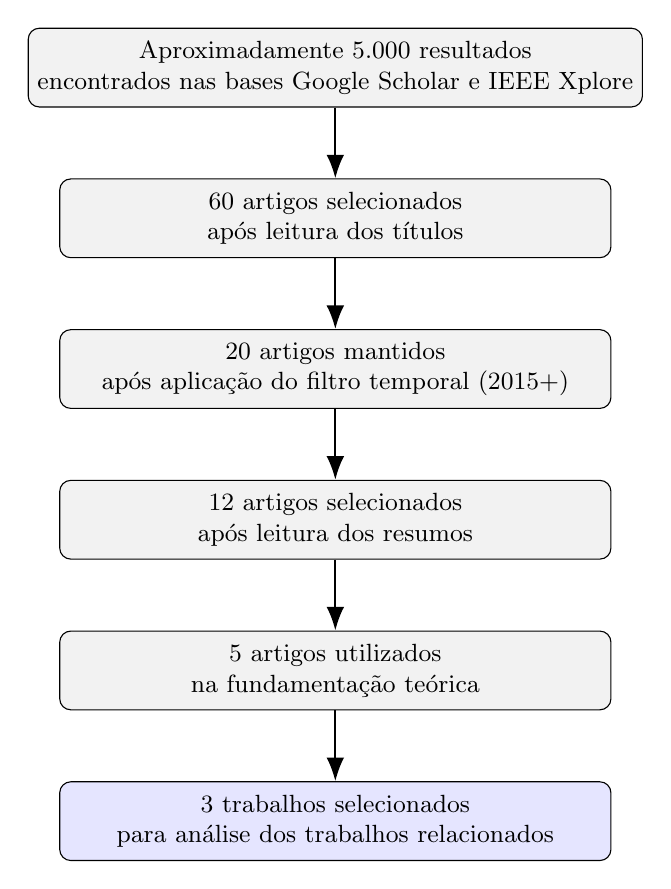
\begin{tikzpicture}[
node distance=0.9cm,
every node/.style={
    align=center,
    font=\small
},
box/.style={
    rectangle,
    rounded corners,
    draw=black,
    minimum width=7cm,
    minimum height=1cm,
    fill=gray!10
},
arrow/.style={
    thick,
    -{Latex[length=3mm]}
}
]

\node[box] (n1) {Aproximadamente 5.000 resultados\\ encontrados nas bases Google Scholar e IEEE Xplore};

\node[box, below=of n1] (n2) {60 artigos selecionados\\ após leitura dos títulos};

\node[box, below=of n2] (n3) {20 artigos mantidos\\ após aplicação do filtro temporal (2015+)};

\node[box, below=of n3] (n4) {12 artigos selecionados\\ após leitura dos resumos};

\node[box, below=of n4] (n5) {5 artigos utilizados\\ na fundamentação teórica};

\node[box, below=of n5, fill=blue!10] (n6) {3 trabalhos selecionados\\ para análise dos trabalhos relacionados};

\draw[arrow] (n1) -- (n2);
\draw[arrow] (n2) -- (n3);
\draw[arrow] (n3) -- (n4);
\draw[arrow] (n4) -- (n5);
\draw[arrow] (n5) -- (n6);

\end{tikzpicture}

\caption{Processo de seleção dos trabalhos utilizados na pesquisa bibliográfica.}
\label{fig:fluxo_bibliografico}

\legend{Fonte: Elaborado pelo autor (2026)}
\end{figure}



A estratégia de seleção adotada permitiu reduzir progressivamente o conjunto inicial de publicações, mantendo apenas trabalhos com elevada aderência técnica ao objetivo da pesquisa e representativos do estado da arte em interpolação de quadros de vídeo e otimização de inferência em GPU.

% ---------------------------------------------------------------
\section{Fundamentos}
\label{sec:fundamentos}

\subsection{Definição de Imagem Digital}

Uma imagem digital pode ser definida como uma função bidimensional $f(x, y)$, onde $x$ e $y$ representam coordenadas espaciais em um plano. De acordo com \citeonline{Gonzalez2009}, quando os valores de $x$, $y$ e a amplitude de $f$ assumem quantidades finitas e discretas, a imagem é caracterizada como digital. Na prática computacional, essa estrutura é representada por uma matriz composta por elementos discretos denominados \textit{pixels} (\textit{picture elements}), que constituem a menor unidade de informação visual de uma imagem.

No modelo de cores RGB (\textit{Red, Green, Blue}), amplamente utilizado em sistemas computacionais, cada pixel é representado por três componentes correspondentes aos canais vermelho, verde e azul. Em implementações convencionais de 8 bits por canal, cada componente assume valores no intervalo $[0,255]$, permitindo a representação de aproximadamente 16,7 milhões de combinações de cores \cite{Szeliski2022}.

A resolução de uma imagem corresponde à quantidade total de pixels que a compõem. Em aplicações de vídeo, o volume de dados cresce rapidamente com o aumento da resolução. Por exemplo, um único quadro em resolução Full HD (1920 $\times$ 1080) contém mais de dois milhões de pixels. Considerando três canais de cor por pixel, a manipulação simultânea de múltiplos quadros pode demandar dezenas de megabytes de memória, tornando o gerenciamento eficiente dos dados um aspecto relevante para algoritmos de processamento de vídeo e interpolação de quadros \cite{Szeliski2022}.

A representação dessas matrizes em linguagem C++ impacta diretamente a performance computacional. Embora conceitualmente bidimensionais, as imagens são frequentemente organizadas na memória como vetores unidimensionais para maximizar o acesso contíguo aos dados. Nesse formato de linearização, a posição de um pixel $(x, y)$ em uma imagem de largura $W$ pode ser obtida pela expressão:

\[
index = (y \times W) + x
\]

Essa organização favorece a localidade espacial de memória e reduz a ocorrência de acessos não contíguos, característica particularmente importante em aplicações de processamento paralelo executadas em GPUs \cite{Szeliski2022,Kirk2023}. Em algoritmos de interpolação de quadros, nos quais milhões de operações são realizadas para cada sequência de vídeo processada, a forma de armazenamento dos pixels pode influenciar diretamente a latência de execução e o consumo de memória.

\subsection{Filtragem Espacial e Convolução Adaptativa}

A convolução constitui uma das operações fundamentais do processamento digital de imagens e da visão computacional moderna. Em sua forma tradicional, um kernel bidimensional percorre toda a imagem aplicando o mesmo conjunto de coeficientes a cada região analisada. Segundo \citeonline{Gonzalez2009}, filtros convolucionais clássicos utilizam coeficientes fixos para executar tarefas como suavização, realce de detalhes, remoção de ruído e detecção de bordas.

Matematicamente, a convolução espacial pode ser interpretada como uma operação de combinação ponderada entre os pixels de uma vizinhança local. Em aplicações convencionais de processamento de imagens, a utilização de um kernel fixo é suficiente, uma vez que a transformação desejada é aplicada uniformemente sobre toda a cena. Entretanto, essa abordagem torna-se limitada em problemas de Interpolação de Quadros de Vídeo (VFI), nos quais diferentes regiões da imagem podem apresentar movimentos distintos entre quadros consecutivos \cite{Szeliski2022}.

Em cenários de VFI, o objetivo não consiste apenas em filtrar uma imagem existente, mas em sintetizar novas informações visuais correspondentes a um instante temporal intermediário. Dessa forma, um único kernel fixo não é capaz de representar adequadamente a variedade de movimentos presentes na cena. Objetos distintos podem deslocar-se em velocidades e direções diferentes, exigindo estratégias adaptativas para estimar corretamente a posição dos pixels no quadro intermediário.

Para superar essa limitação, surgem as convoluções adaptativas, nas quais os coeficientes do kernel deixam de ser constantes e passam a ser estimados individualmente para cada pixel da imagem. Conforme proposto por \citeonline{Niklaus2017}, os coeficientes desses kernels funcionam como indicadores de amostragem, determinando de quais posições espaciais nos quadros de entrada as informações devem ser extraídas para sintetizar o pixel correspondente ao instante intermediário ($t+0.5$).

Essa estratégia permite incorporar implicitamente informações de movimento durante o próprio processo de síntese da imagem. Em vez de realizar uma etapa explícita de estimativa de fluxo óptico seguida de reconstrução do quadro, a convolução adaptativa unifica ambas as tarefas em uma única operação. Como resultado, o modelo passa a aprender simultaneamente onde buscar informações e como combiná-las, reduzindo a complexidade do pipeline e possibilitando a geração de quadros intermediários com elevada qualidade visual \cite{Niklaus2021}.

\subsection{Fluxo Óptico Explícito vs. Kernels de Movimento Implícito}

Grande parte dos métodos modernos de Interpolação de Quadros de Vídeo (VFI) baseia-se na estimativa de movimento entre quadros consecutivos. Nesse contexto, o conceito de fluxo óptico desempenha papel fundamental ao descrever o deslocamento aparente dos pixels entre duas imagens ao longo do tempo. Formalmente, o fluxo óptico pode ser representado por um campo vetorial denso, no qual cada pixel possui um vetor $(u,v)$ indicando sua direção e magnitude de deslocamento \cite{Szeliski2022}.

Entre os modelos contemporâneos mais relevantes para estimativa de fluxo óptico destaca-se o RAFT (\textit{Recurrent All-Pairs Field Transforms}), proposto por \citeonline{Teed2020}. O modelo constrói volumes de correlação entre todos os pares de pixels das imagens de entrada e utiliza um mecanismo recorrente para refinar iterativamente os vetores de movimento. Essa estratégia permite atingir elevados níveis de precisão, tornando o RAFT uma das principais referências da área de visão computacional.

Após a estimativa do fluxo óptico, métodos tradicionais de VFI realizam uma etapa adicional denominada \textit{warping}, responsável por deformar ou reposicionar os pixels dos quadros originais de acordo com os vetores calculados. Embora eficaz, essa abordagem pode apresentar dificuldades em regiões de oclusão, desoclusão ou movimentos complexos, nas quais determinados pixels tornam-se visíveis ou invisíveis entre quadros consecutivos \cite{Teed2020,Szeliski2022}.

Uma alternativa a esse paradigma consiste na utilização de kernels de movimento implícito, abordagem adotada pelos métodos baseados em convolução adaptativa. Nesse cenário, o movimento não é representado explicitamente por vetores de deslocamento. Em vez disso, a rede neural aprende diretamente um conjunto de coeficientes responsáveis por determinar como os pixels dos quadros de entrada devem ser combinados para sintetizar o valor correspondente ao quadro intermediário \cite{Niklaus2017}.

Sob essa perspectiva, os pesos do kernel passam a codificar implicitamente informações de movimento e correspondência espacial. Em vez de calcular uma "seta" indicando o deslocamento de cada pixel, o modelo aprende quais amostras locais devem ser utilizadas e qual contribuição cada uma delas terá na reconstrução do novo quadro. Dessa forma, a estimativa de movimento e a síntese da imagem tornam-se partes de uma única operação computacional.

Essa unificação simplifica o \textit{pipeline} de processamento e elimina a necessidade de etapas explícitas de fluxo óptico e \textit{warping}. Além disso, reduz a propagação de erros entre estágios sucessivos do algoritmo, característica que contribuiu para a popularização das abordagens baseadas em convolução adaptativa na literatura recente de interpolação de quadros de vídeo \cite{Niklaus2017,Niklaus2021}.

\subsection{Eficiência via Convoluções Separáveis}

O principal desafio das abordagens baseadas em convolução adaptativa está relacionado ao tamanho dos kernels necessários para representar movimentos de grande magnitude. Em métodos de interpolação de quadros, cada pixel do quadro intermediário pode depender de uma ampla região dos quadros de entrada, exigindo filtros com dimensões elevadas. Consequentemente, o custo computacional cresce rapidamente à medida que o tamanho do kernel aumenta \cite{Niklaus2017}.

Em uma convolução bidimensional convencional, um kernel de dimensão $N \times N$ contém $N^2$ coeficientes. Isso significa que cada pixel processado requer a combinação de $N^2$ amostras da imagem de entrada. Para um kernel de $51 \times 51$, por exemplo, são necessárias 2.601 operações de combinação para cada pixel sintetizado. Considerando imagens em resolução HD ou Full HD, esse custo torna-se extremamente elevado tanto em processamento quanto em consumo de memória \cite{Niklaus2017,Niklaus2021}.

A técnica de convolução separável busca reduzir essa complexidade explorando uma propriedade matemática específica de determinados filtros. Em vez de representar o kernel como uma matriz bidimensional completa, ele é decomposto em dois filtros unidimensionais independentes: um filtro vertical e um filtro horizontal. Matematicamente, essa decomposição pode ser expressa como:

\[
K = v \cdot h^{T}
\]

onde $v$ representa o vetor vertical e $h$ representa o vetor horizontal. Dessa forma, a convolução bidimensional passa a ser executada em duas etapas sucessivas de convolução unidimensional \cite{Niklaus2017}.

Como consequência, o número de operações deixa de crescer quadraticamente e passa a crescer linearmente em relação ao tamanho do filtro. Enquanto uma convolução tradicional exige aproximadamente $N^2$ operações por pixel, a versão separável requer apenas $N + N = 2N$ operações. Para um filtro de dimensão $51 \times 51$, isso representa uma redução de 2.601 para apenas 102 operações por pixel.

Essa diferença possui impacto direto na viabilidade computacional do algoritmo. A redução do número de coeficientes diminui a quantidade de acessos à memória, reduz o volume de dados intermediários armazenados durante a inferência e aumenta o potencial de paralelização em arquiteturas modernas de GPU. Como resultado, convoluções separáveis tornam possível utilizar kernels de grande alcance espacial sem que o custo computacional se torne proibitivo \cite{Niklaus2017,Kirk2023}.

No contexto deste trabalho, essa propriedade é particularmente relevante, pois a redução da complexidade matemática influencia diretamente a latência de execução e o consumo de memória VRAM durante a inferência. Dessa forma, a separabilidade dos kernels constitui o principal mecanismo que viabiliza a execução de modelos de interpolação de quadros em GPUs de consumo com capacidade limitada de memória.


\subsection{Implementação de Baixo Nível e I/O de Vídeo}

O desenvolvimento de aplicações de processamento de vídeo em alto desempenho exige atenção não apenas aos algoritmos empregados, mas também à forma como os dados são organizados e transferidos entre os diferentes níveis da arquitetura computacional. Nesse contexto, a linguagem C++ é amplamente utilizada em aplicações de visão computacional e computação de alto desempenho por oferecer controle explícito sobre a alocação de memória, estruturas de dados e gerenciamento de recursos do sistema \cite{Kirk2023}.

Em aplicações aceleradas por GPU, os dados normalmente são armazenados inicialmente na memória principal do sistema (Host) e posteriormente transferidos para a memória de vídeo da placa gráfica (Device). Essas transferências ocorrem através do barramento PCI Express (PCIe), cuja largura de banda é significativamente inferior à largura de banda interna da memória da GPU. Consequentemente, movimentações excessivas de dados podem se tornar um gargalo relevante para o desempenho da aplicação \cite{NvidiaCUDA2025}.

Para minimizar esse problema, é comum organizar os dados em regiões contíguas de memória antes da transferência para o dispositivo gráfico. Essa estratégia melhora a localidade espacial dos acessos, reduz a fragmentação dos dados e favorece operações de leitura e escrita mais eficientes tanto na CPU quanto na GPU \cite{Kirk2023}.

No contexto deste trabalho, os quadros de vídeo serão inicialmente carregados utilizando bibliotecas especializadas de entrada e saída de mídia. Após a decodificação, os dados serão reorganizados em estruturas lineares adequadas para processamento paralelo, permitindo transferências eficientes entre memória principal e memória gráfica. Essa etapa é particularmente importante em aplicações de interpolação de quadros, uma vez que múltiplas imagens de alta resolução precisam ser mantidas simultaneamente em memória durante o processo de inferência.


\subsection{Inferência Desacoplada via ONNX Runtime}

O Open Neural Network Exchange (ONNX) consiste em um formato intermediário padronizado para representação de modelos de aprendizado profundo, permitindo interoperabilidade entre diferentes frameworks de treinamento e ambientes de inferência \cite{ONNX2026}. Nesse ecossistema, o ONNX Runtime atua como um mecanismo otimizado de execução, possibilitando a inferência de redes neurais sem dependência direta do framework originalmente utilizado durante o treinamento.

No contexto desta pesquisa, a utilização do ONNX Runtime possui relevância arquitetural, pois permite desacoplar a inferência do ecossistema Python/PyTorch, reduzindo \textit{overheads} relacionados à abstração de alto nível e ao gerenciamento adicional de memória. Além disso, a biblioteca oferece integração nativa com provedores de execução CUDA, permitindo que os tensores permaneçam alocados diretamente na VRAM da GPU durante o pipeline de processamento.

Essa abordagem é particularmente importante para a hipótese investigada neste trabalho, uma vez que a redução de transferências desnecessárias entre memória principal e memória de vídeo constitui um fator relevante para mitigação do gargalo conhecido como \textit{Memory Wall}. Dessa forma, o ONNX Runtime atua não apenas como ferramenta de execução, mas como componente estrutural da estratégia de otimização proposta.


\subsection{Arquitetura de Decomposição e Garantia de Separabilidade}

A viabilidade técnica de utilizar kernels de grandes dimensões (como $51 \times 51$) depende da garantia matemática de separabilidade. Para que uma matriz $K$ seja separável, ela deve obrigatoriamente possuir Posto 1 (\textit{Rank-1}), permitindo sua decomposição no produto externo de dois vetores unidimensionais: $K = v \cdot h^T$.

O modelo SepConv resolve esse desafio diretamente em sua arquitetura de rede neural através de uma \textbf{bifurcação na camada de saída}. Em vez de estimar os $N^2$ elementos de uma matriz bidimensional, a rede possui duas ramificações independentes que inferem, simultaneamente, um vetor vertical $v$ ($N \times 1$) e um vetor horizontal $h$ ($1 \times N$). 

Ao forçar essa estrutura, o algoritmo garante que o kernel resultante seja sempre separável, eliminando erros de aproximação que ocorreriam em uma decomposição analítica \textit{a posteriori}. Para a implementação em C++, essa característica é fundamental: o sistema recebe da rede neural apenas $2N$ valores por pixel, permitindo que a operação de convolução seja executada em dois passos lineares sequenciais, reduzindo drasticamente o esforço computacional e a ocupação de memória sem perda de precisão matemática em relação ao modelo bidimensional pretendido.

\subsection{Arquitetura de GPU e o Gargalo de Memória (\textit{Memory Wall})}

A execução de modelos profundos de visão computacional em hardware de consumo não é apenas um desafio aritmético, mas fundamentalmente um problema de tráfego de dados. Segundo a teoria arquitetural apresentada por \citeonline{Hennessy2022}, os sistemas modernos sofrem com o chamado \textit{Memory Wall} (Muro da Memória), um fenômeno no qual a capacidade de processamento cresce em ritmo significativamente superior ao aumento da largura de banda da memória. Como consequência, em diversas aplicações computacionais, especialmente aquelas intensivas em dados, o tempo gasto movimentando informações entre memória e unidades de processamento frequentemente supera o tempo efetivamente dedicado aos cálculos.

No ecossistema de Unidades de Processamento Gráfico (GPUs), essa dinâmica é regida pelo modelo de execução \textit{Single Instruction, Multiple Threads} (SIMT). Conforme descrito por \citeonline{Kirk2023}, a eficiência máxima de uma GPU é alcançada quando os acessos à memória ocorrem de forma coalescida e contígua, permitindo que múltiplas threads compartilhem operações de leitura e escrita de maneira eficiente. Transferências excessivas pelo barramento PCI Express (PCIe), bem como realocações frequentes de grandes tensores na memória global da GPU, podem introduzir gargalos significativos e reduzir a taxa efetiva de processamento \cite{NvidiaCUDA2025}.

Dessa forma, a escolha metodológica de transpor kernels tradicionais para convoluções separáveis --- reduzindo o armazenamento temporal de $O(N^2)$ para $O(N)$ --- transcende a mera economia de operações matemáticas de ponto flutuante. A separabilidade matemática reduz o \textit{footprint} (pegada) espacial da inferência diretamente na memória global da GPU, diminuindo a quantidade de dados movimentados e reduzindo a pressão sobre os subsistemas de memória. Essa característica é particularmente relevante considerando que, essa característica é particularmente relevante considerando que, segundo a Steam Hardware Survey, placas de vídeo com 8 GB de VRAM representam atualmente a configuração individual mais comum entre os usuários da plataforma \cite{SteamSurvey2026}. Dessa forma, a redução do consumo de memória torna-se um requisito prático para ampliar a acessibilidade de técnicas avançadas de interpolação de quadros em ambientes domésticos e em hardware de consumo.

Consequentemente, a redução do consumo de memória proporcionada pelas convoluções separáveis não apenas melhora a eficiência computacional, mas também contribui para evitar limitações impostas pela capacidade física da VRAM, fundamentando teoricamente a hipótese de redução de latência e viabilização da inferência em GPUs comerciais de capacidade moderada.

\subsection{Métricas de Avaliação Objetiva de Qualidade}

A validação de algoritmos de Interpolação de Quadros de Vídeo (VFI) exige a comparação entre o quadro sintetizado ($I_{sint}$) e o quadro real de referência ($I_{real}$), também denominado \textit{ground truth}. Para quantificar objetivamente a fidelidade visual das imagens geradas, este trabalho utilizará duas métricas amplamente adotadas na literatura de processamento de imagens e visão computacional: Peak Signal-to-Noise Ratio (PSNR) e Structural Similarity Index (SSIM).

\textbf{1. Peak Signal-to-Noise Ratio (PSNR):}

O PSNR é uma das métricas mais tradicionais para avaliação da qualidade de imagens reconstruídas ou comprimidas. Sua formulação é baseada no Erro Quadrático Médio (\textit{Mean Squared Error} -- MSE), que mede a diferença pixel a pixel entre a imagem sintetizada e a imagem de referência \cite{Hore2010}.

Matematicamente, o PSNR é definido como:

\begin{equation}
    PSNR = 10 \cdot \log_{10}
    \left(
    \frac{MAX_I^2}{MSE}
    \right)
\end{equation}

onde $MAX_I$ representa o valor máximo possível de intensidade de um pixel, assumindo normalmente o valor 255 em imagens de 8 bits.

Valores mais elevados de PSNR indicam menor erro de reconstrução e, consequentemente, maior proximidade numérica entre a imagem gerada e a imagem original. Entretanto, embora seja simples e computacionalmente eficiente, essa métrica apresenta limitações perceptuais, pois considera apenas diferenças absolutas entre pixels, sem levar em conta a forma como o sistema visual humano interpreta estruturas, texturas e padrões espaciais \cite{Hore2010}.

\vspace{0.3cm}

\textbf{2. Structural Similarity Index (SSIM):}

Para contornar as limitações perceptuais do PSNR, \citeonline{Wang2004} propuseram o \textit{Structural Similarity Index} (SSIM), uma métrica baseada na hipótese de que o sistema visual humano é mais sensível à preservação de estruturas locais do que a diferenças absolutas de intensidade.

O SSIM compara regiões correspondentes entre duas imagens considerando simultaneamente três componentes fundamentais:

\begin{itemize}
    \item luminância;
    \item contraste;
    \item estrutura.
\end{itemize}

O resultado é um valor normalmente compreendido no intervalo $[0,1]$, onde valores próximos de 1 indicam elevada similaridade estrutural entre as imagens comparadas.

Em aplicações de interpolação de quadros, o SSIM é particularmente relevante por ser capaz de identificar degradações visuais frequentemente observadas em quadros sintetizados, como borramento de bordas, perda de detalhes finos e artefatos decorrentes de erros de estimativa de movimento. Por esse motivo, a métrica é amplamente utilizada na literatura contemporânea de VFI como complemento ao PSNR \cite{Niklaus2017,Niklaus2021}.

A utilização conjunta de PSNR e SSIM permite avaliar tanto a precisão numérica quanto a qualidade perceptual das imagens geradas. Dessa forma, torna-se possível analisar os impactos das otimizações propostas neste trabalho não apenas sobre a latência e o consumo de memória, mas também sobre a fidelidade visual dos quadros sintetizados.


\subsection{Mensuração de Desempenho Computacional}

Além da qualidade visual dos quadros sintetizados, a avaliação de algoritmos de Interpolação de Quadros de Vídeo (VFI) envolve aspectos relacionados à eficiência computacional. Em aplicações práticas, especialmente em sistemas de tempo real, a qualidade da imagem deve ser analisada em conjunto com o custo necessário para produzi-la, uma vez que algoritmos visualmente precisos podem apresentar inviabilidade operacional devido ao elevado consumo de recursos computacionais \cite{Kirk2023}.

Nesse contexto, duas métricas são frequentemente empregadas na literatura para caracterizar o desempenho de sistemas acelerados por GPU: a latência de processamento e o consumo de memória. A latência representa o tempo necessário para que uma determinada operação seja concluída, influenciando diretamente a capacidade do sistema de processar sequências de vídeo em tempo real. Em aplicações de visão computacional, reduções de poucos milissegundos por quadro podem resultar em aumentos significativos na taxa efetiva de processamento (\textit{throughput}) \cite{Hennessy2022}.

Por sua vez, o consumo de memória constitui um fator limitante para a execução de modelos de aprendizado profundo em hardware de consumo. A necessidade de armazenar simultaneamente quadros de entrada, ativações intermediárias e parâmetros do modelo pode levar ao esgotamento da memória disponível, inviabilizando a inferência mesmo quando a capacidade de processamento da GPU permanece ociosa. Por esse motivo, a utilização eficiente da VRAM tornou-se um aspecto relevante no desenvolvimento de aplicações modernas de inteligência artificial \cite{NvidiaCUDA2025}.

No contexto da interpolação de quadros baseada em convoluções adaptativas separáveis, a redução da complexidade espacial representa um dos principais fatores que podem contribuir para a diminuição do consumo de memória e para a melhoria da eficiência geral do sistema. Dessa forma, a análise conjunta de métricas de qualidade visual e desempenho computacional permite uma avaliação mais abrangente dos benefícios e limitações da abordagem investigada neste trabalho.
% ---------------------------------------------------------------
\section{Trabalhos relacionados}
\label{sec:trabalhos_relacionados}

Nesta seção, são apresentados três trabalhos recentes que abordam o desafio da Interpolação de Quadros de Vídeo (VFI). A seleção prioriza métodos que, assim como esta pesquisa, buscam o equilíbrio entre a fidelidade visual e a eficiência no processamento de grandes deslocamentos de pixels.

\subsection{Trabalho 1: Revisiting Adaptive Convolutions for Video Frame Interpolation}

\citeonline{Niklaus2021} abordou o problema da complexidade crescente das redes neurais de interpolação, que muitas vezes exigem recursos computacionais excessivos para ganhos marginais de qualidade. Para resolvê-lo, o autor propôs uma revisitação ao método de convoluções adaptativas, introduzindo melhorias sutis na arquitetura de estimativa de kernel. A metodologia baseou-se no refinamento do modelo SepConv original, otimizando a forma como os filtros $1D$ são gerados. Os resultados mostraram que modelos baseados em kernels podem atingir métricas de PSNR e SSIM próximas ao estado da arte com estruturas mais simples. No entanto, a solução ainda depende de frameworks de alto nível (PyTorch) para execução. O presente trabalho diferencia-se por investigar experimentalmente a inferência pura baseada nesses conceitos em C++, focando na eliminação do \textit{overhead} inerente às bibliotecas de aprendizado profundo na alocação de GPU.

\subsection{Trabalho 2: Motion-Aware Video Frame Interpolation}

\citeonline{HAN2024106433} abordaram o problema da representação inadequada de movimentos complexos em métodos tradicionais de interpolação de quadros, especialmente em cenários com deslocamentos rápidos, mudanças abruptas de direção e regiões de oclusão. Para enfrentar essa limitação, os autores propuseram uma arquitetura baseada em modelagem de movimento multi-escala, capaz de capturar informações espaciais e temporais em diferentes níveis de resolução.

A metodologia combina a extração hierárquica de características com mecanismos de estimativa de movimento que integram informações provenientes de múltiplas escalas da imagem. Essa estratégia permite representar movimentos de grande amplitude sem depender exclusivamente de kernels locais ou de campos de fluxo óptico densos, reduzindo artefatos temporais frequentemente observados em sequências complexas.

Os resultados experimentais demonstraram melhorias na preservação da consistência temporal e na qualidade visual dos quadros sintetizados quando comparados a métodos anteriores de interpolação. Em particular, os autores reportam redução de artefatos em regiões com movimentos rápidos e melhor reconstrução de detalhes estruturais.

Entretanto, a arquitetura proposta prioriza a qualidade visual e a robustez da representação de movimento, sem foco específico na redução do consumo de memória ou na otimização da inferência para hardware de consumo. O presente trabalho diferencia-se ao investigar experimentalmente como a separabilidade de kernels e a inferência desacoplada via ONNX Runtime podem contribuir para reduzir a latência e o consumo de VRAM em GPUs comerciais, mantendo níveis aceitáveis de fidelidade visual.


\subsection{Trabalho 3: RAFT: Recurrent All-Pairs Field Transforms for Optical Flow}

\citeonline{Teed2020} abordou a precisão na estimativa de movimento, um problema seminal para a síntese de novos quadros. Para resolvê-lo, propuseram o modelo RAFT, que utiliza uma arquitetura recorrente para atualizar campos de fluxo óptico através de volumes de correlação de todos os pares de pixels. A metodologia utiliza iterações sucessivas para refinar o movimento detectado. Os resultados estabeleceram um novo estado da arte em termos de precisão de vetores. No entanto, a solução apresenta alta latência e exige GPUs de alto desempenho, limitando severamente a viabilidade em cenários comuns. O presente trabalho diferencia-se por adotar a convolução adaptativa como uma alternativa mais contida ao fluxo óptico denso do RAFT, priorizando a performance em GPU e a otimização do consumo de VRAM através de uma inferência nativa.

\vspace{0.5cm}

\begin{table}[htb]
    \centering
    \caption{Comparação entre trabalhos relacionados e a abordagem proposta}
    \label{tab:trabalhos_relacionados}
    \begin{tabularx}{\textwidth}{l|X|X|X}
        \toprule
        \textbf{Trabalho} & \textbf{Estratégia VFI} & \textbf{Tecnologia} & \textbf{Foco / Diferencial} \\
        \midrule
        Niklaus (2021) & Convolução Adaptativa Refinada & Redes Neurais (PyTorch) & Qualidade visual elevada com arquitetura baseada em kernels adaptativos separáveis. \\
        \midrule
        Han et al. (2024) & Modelagem de Movimento Multi-Escala & Pirâmide Hierárquica e Fluxo Intermediário & Melhor representação de movimentos complexos e redução de artefatos temporais. \\
        \midrule
        RAFT (2020) & Fluxo Óptico Recorrente & Volumes de Correlação & Alta precisão na estimativa de movimento com elevado custo computacional. \\
        \midrule
        \textbf{Este trabalho} & \textbf{Inferência SepConv em Baixo Nível} & \textbf{C++ / CUDA / ONNX Runtime} & \textbf{Redução de latência e consumo de VRAM em GPUs de consumo mantendo qualidade visual adequada.} \\
        \bottomrule
    \end{tabularx}
    \legend{Fonte: Elaborado pelo autor (2026)}
\end{table}


% ===============================================================
% CAPÍTULO 3 - DESENVOLVIMENTO
% ===============================================================
\chapter{Desenvolvimento}
\label{cap:desenvolvimento}

Neste capítulo, apresenta-se a solução proposta para o problema identificado, bem como o cronograma de trabalho previsto para o desenvolvimento completo do projeto no TCC2.

% ---------------------------------------------------------------
\section{Solução proposta}
\label{sec:solucao}

A solução proposta para investigar a viabilidade técnica e a eficiência das convoluções adaptativas separáveis consiste no desenvolvimento de um motor de inferência customizado para Interpolação de Quadros de Vídeo (VFI). O foco é transpor a etapa de inferência do modelo SepConv para um ambiente otimizado em GPU. A descrição detalhada do projeto segue abaixo:

\begin{itemize}
    \item \textbf{Visão geral da solução}: Será desenvolvida uma ferramenta de software de linha de comando (CLI) focada puramente na inferência do modelo SepConv. O sistema processará pares de quadros de um vídeo de entrada, utilizará pesos pré-treinados para gerar os \textit{kernels} de movimento, sintetizará o quadro intermediário e compilará um novo vídeo de saída, registrando os picos de uso de VRAM integrando a API da \textit{NVIDIA Management Library} (NVML) e a latência da execução via eventos CUDA.

    \item \textbf{Arquitetura}: O sistema opera em um fluxo de dados (\textit{pipeline}) de cinco estágios:
    \begin{enumerate}
        \item \textbf{I/O (Host):} Leitura e decodificação dos quadros na RAM do sistema via OpenCV;
        \item \textbf{Transferência (Host-to-Device):} Envio dos dados linearizados da RAM para a VRAM da GPU;
        \item \textbf{Inferência (ONNX Runtime):} Processamento do modelo pré-treinado SepConv para gerar os vetores separados 1D para cada pixel, mantendo-os alocados nativamente na GPU;
        \item \textbf{Convolução (CUDA):} Aplicação paralela da convolução separável $O(N)$ utilizando blocos e \textit{threads} CUDA nativamente na VRAM para compor o quadro final;
        \item \textbf{Retorno e Escrita:} Transferência apenas do quadro gerado final de volta para o Host e codificação do vídeo.
    \end{enumerate}

    \item \textbf{Tecnologias e ferramentas}: O controle do fluxo será desenvolvido em \textbf{C++17}. Para a leitura e decodificação do vídeo, optou-se pela biblioteca \textbf{OpenCV (C++ API)}. O motor de inferência dos filtros será a biblioteca \textbf{ONNX Runtime} (operando via provedor CUDA), enquanto a aplicação matemática intensiva e paralela sobre a imagem fará uso das APIs nativas \textbf{NVIDIA CUDA C++}.

    \item \textbf{Funcionalidades principais}: A ferramenta carregará o modelo `.onnx`, executará a predição quadro a quadro, aferirá os tempos de latência em milissegundos utilizando as medições do ecossistema NVIDIA e exportará um consolidado do pico de memória VRAM registrado.

    \item \textbf{Metodologia de desenvolvimento}: Será adotada uma abordagem de ciclos iterativos de otimização (\textit{Profiling-Driven Development}). O protótipo validará as transferências básicas de memória e, progressivamente, focará em medir o comportamento da placa de vídeo e o esgotamento dos seus 8 GB ao aplicar o kernel de forma escalonada.

    \item \textbf{Critérios de validação e Mensuração de Hardware}: O sucesso da eficiência será avaliado contrastando os resultados da arquitetura proposta com a \textit{baseline} padrão em Python/PyTorch do mesmo modelo. A coleta de dados do consumo de VRAM será efetuada através da \textit{NVIDIA Management Library} (NVML) e utilitários como o \textit{Nsight Systems}, garantindo a precisão ao isolar o processamento principal. A latência será aferida no código C++ através de eventos da API (\texttt{cudaEventRecord}), isolando o tempo real de processamento matemático paralelo na GPU.
    
    \item \textbf{Seleção de Dataset}: A avaliação experimental de qualidade visual e consumo associado será conduzida usando fragmentos do \textit{dataset} \textbf{Vimeo-90K}, escalonados e ajustados para a resolução de testes.
\end{itemize}

% ---------------------------------------------------------------
\section{Cronograma de trabalho}
\label{sec:cronograma}

O cronograma a seguir apresenta, no formato de diagrama de Gantt, as atividades previstas para o desenvolvimento do TCC2, distribuídas ao longo das semanas do semestre.

\begin{figure}[htb]
    \centering
    \caption{Cronograma de atividades -- Diagrama de Gantt}
    \label{fig:gantt}

    \resizebox{\textwidth}{!}{
    \begin{ganttchart}[
        hgrid,
        vgrid,
        x unit=0.75cm,
        y unit title=0.6cm,
        y unit chart=0.7cm,
        title height=1,
        bar height=0.5,
        bar label font=\tiny,
        title label font=\small,
        milestone label font=\tiny\itshape,
        group label font=\scriptsize\bfseries,
        bar/.append style={fill=senacblue!40},
        group/.append style={draw=black, fill=senacblue!70},
        milestone/.append style={fill=red!70},
    ]{1}{16}

        % Semanas
        \gantttitle{Semanas}{16} \\
        \gantttitlelist{1,...,16}{1} \\

        % Fase 1
        \ganttgroup{Fase 1: Planejamento}{1}{4} \\
        \ganttbar{Revisão bibliográfica}{1}{4} \\
        \ganttbar{Arquitetura da solução}{2}{4} \\
        \ganttbar{Planejamento experimental}{3}{4} \\
        \ganttmilestone{Entrega TCC1}{4} \\

        % Fase 2
        \ganttgroup{Fase 2: Desenvolvimento}{5}{11} \\
        \ganttbar{Módulo de I/O}{5}{6} \\
        \ganttbar{Integração ONNX Runtime}{6}{8} \\
        \ganttbar{Kernels CUDA}{8}{10} \\
        \ganttbar{Integração do pipeline}{10}{11} \\
        \ganttmilestone{Protótipo funcional}{11} \\

        % Fase 3
        \ganttgroup{Fase 3: Validação}{12}{16} \\
        \ganttbar{Extração de métricas}{12}{14} \\
        \ganttbar{Avaliação PSNR/SSIM}{13}{15} \\
        \ganttbar{Análise dos resultados}{14}{15} \\
        \ganttmilestone{Validação experimental}{15} \\

        % Escrita
        \ganttgroup{Documentação}{1}{16} \\
        \ganttbar{Redação e revisão do TCC}{1}{16} \\
        \ganttmilestone{Entrega final}{16}

        % Dependências
        \ganttlink{elem2}{elem3}
        \ganttlink{elem3}{elem4}
        \ganttlink{elem6}{elem7}
        \ganttlink{elem7}{elem8}
        \ganttlink{elem8}{elem9}
        \ganttlink{elem10}{elem11}

    \end{ganttchart}
    }

    \legend{Fonte: Elaborado pelo autor (2026)}
\end{figure}

% ---------------------------------------------------------------
% ELEMENTOS PÓS-TEXTUAIS
% ---------------------------------------------------------------
\postextual

% ===============================================================
% CAPÍTULO 4 - REFERÊNCIAS BIBLIOGRÁFICAS
% ===============================================================
% As referências bibliográficas são geradas automaticamente a partir
% do arquivo bibliografia.bib, seguindo o padrão ABNT (NBR 6023).
%
% COMO CITAR no texto:
%   \cite{chave}         -> (SOBRENOME, ano) — citação indireta
%   \citeonline{chave}   -> Sobrenome (ano) — citação direta no texto
%
% TIPOS DE REFERÊNCIA no arquivo .bib:
%   @book        -> Livros
%   @article     -> Artigos de periódicos
%   @inproceedings -> Artigos em anais de eventos
%   @mastersthesis -> Dissertações de mestrado
%   @phdthesis   -> Teses de doutorado
%   @misc        -> Sites, vídeos e outros materiais
%   @manual      -> Documentação técnica
%
% Veja o arquivo bibliografia.bib para exemplos de cada tipo.
% ---------------------------------------------------------------
\bibliography{bibliografia}

% ---------------------------------------------------------------
% APÊNDICES (se necessário)
% ---------------------------------------------------------------
% \begin{apendicesenv}
% \partapendices
%
% \chapter{Nome do Apêndice}
% \label{ap:apendice1}
%
% Conteúdo do apêndice (material elaborado pelo próprio autor).
%
% \end{apendicesenv}

% ---------------------------------------------------------------
% ANEXOS (se necessário)
% ---------------------------------------------------------------
% \begin{anexosenv}
% \partanexos
%
% \chapter{Nome do Anexo}
% \label{an:anexo1}
%
% Conteúdo do anexo (material de terceiros).
%
% \end{anexosenv}

\end{document}